\documentclass[preprint,12pt,number]{elsarticle}

\usepackage{amsmath,amssymb,amsfonts}
\usepackage{booktabs}
\usepackage{tabularx}
\usepackage{graphicx}
\usepackage{subcaption}
\usepackage{float}
\usepackage{lineno}
\usepackage{hyperref}
\hypersetup{hidelinks}

\journal{Ain Shams Engineering Journal}
\graphicspath{{images/}}
\biboptions{sort&compress}

\begin{document}

\begin{frontmatter}

\title{PinPoint: Synchronization-Aware and Explainable Audio--Visual Deepfake Detection}

\author{Author information withheld for double-anonymized review}

\begin{abstract}
Audio--visual deepfakes create a forensic challenge because a detector must identify manipulated media while also exposing evidence that can be inspected by human reviewers. Existing multimodal detectors often fuse acoustic and visual features without explicitly constraining whether the learned interaction reflects temporal synchrony between speech and facial motion. This paper presents PinPoint, a synchronization-aware audio--visual detector designed to make cross-modal alignment both predictive and auditable. PinPoint combines an explainability-compatible ResNet-18 visual encoder, a convolutional Gated Recurrent Unit audio encoder, stacked gated cross-attention blocks, a three-stage curriculum, and a multi-component synchronization loss that encourages aligned real samples to produce diagonal, concentrated, and temporally smooth audio-to-video attention maps. On a unified benchmark constructed from LAV-DF and FakeAVCeleb, PinPoint achieves 97.47\% accuracy over 26,097 test samples, with macro F1 of 0.9680 and fake-class F1 of 0.9825. Ablation experiments show that removing the gate, synchronization loss, or curriculum reduces accuracy to 58.35\%, 75.47\%, and 81.44\%, respectively. A multimodal explainable artificial intelligence analysis using Integrated Gradients, Layer-wise Relevance Propagation, SHAP, LIME, attention visualization, counterfactuals, and Testing with Concept Activation Vectors links the predictions to mouth-region, acoustic-feature, and lip-sync evidence. These results indicate that synchrony-aware supervision can improve deepfake detection accuracy while making model behavior easier to audit.
\end{abstract}

\begin{keyword}
Deepfake detection \sep Audio--visual fusion \sep Explainable artificial intelligence \sep Synchronization loss \sep Cross-attention \sep Curriculum learning
\end{keyword}

\end{frontmatter}

\linenumbers

\section{Introduction}
\label{sec:introduction}

Generative models can now alter speech, facial identity, and lip motion with a realism that makes manipulated videos difficult to assess by visual inspection alone. This changes deepfake detection from a simple binary classification problem into a forensic decision problem: the detector must be accurate, but it must also provide evidence that can be reviewed when the output affects journalism, legal evidence, political communication, or personal reputation. Recent surveys of passive multimodal deepfake detection emphasize the same pressure point: robustness, generalization, and interpretability remain open concerns when detectors are exposed to new manipulation pipelines and post-processing conditions \cite{nguyen2024survey}.

Many early detectors exploited visual artifacts such as blending boundaries, texture mismatch, lighting inconsistency, or high-frequency synthesis traces. These cues can work well when training and test data share the same generation process, but they become less reliable as synthesis pipelines improve and compression removes fragile artifacts. Audio-only detectors face a similar problem because spectral synthesis artifacts may disappear as voice conversion and text-to-speech systems improve. Audio--visual deepfakes, however, also create a more structural cue: the relationship between what is spoken and how the face moves while speaking.

Synchronization cues are attractive because they are tied to the physics and timing of human communication. A manipulated video may preserve plausible frames and plausible audio independently while still disrupting the temporal correspondence between phonetic events, mouth openings, and facial motion. Prior work has shown that audio--visual dissonance, lip motion, and multimodal representation learning can improve detection \cite{chugh2020notmade,haliassos2021lips,raza2023multimodaltrace,javed2025avsff}. Yet fusion by itself does not guarantee synchrony-aware reasoning. A cross-attention model can still learn shortcut correlations if the training objective only rewards final real/fake classification.

This limitation matters for forensic use. If a detector marks a video as fake, an examiner should be able to ask whether the model relied on mouth-region evidence, acoustic timing, audio--visual mismatch, or unrelated visual artifacts. Post-hoc saliency maps can help, but they do not prove that the model learned a synchronization concept. PinPoint addresses this gap by making synchronization part of the optimization target and then auditing the trained model with multiple explanation methods.

We introduce PinPoint, an interpretable audio--visual architecture for deepfake detection. Figure~\ref{fig:overview} summarizes the proposed framework. PinPoint processes 30-frame video clips and Mel-frequency cepstral coefficient (MFCC) audio sequences with modality-specific encoders, fuses them with gated cross-attention, and trains the attention structure with a synchronization loss applied to aligned real samples. The same attention map used for prediction therefore receives a task-specific interpretation: diagonal structure indicates that audio timesteps attend to temporally corresponding video frames, while diffuse or off-diagonal structure signals weaker audio--visual correspondence.

\begin{figure}[H]
\centering
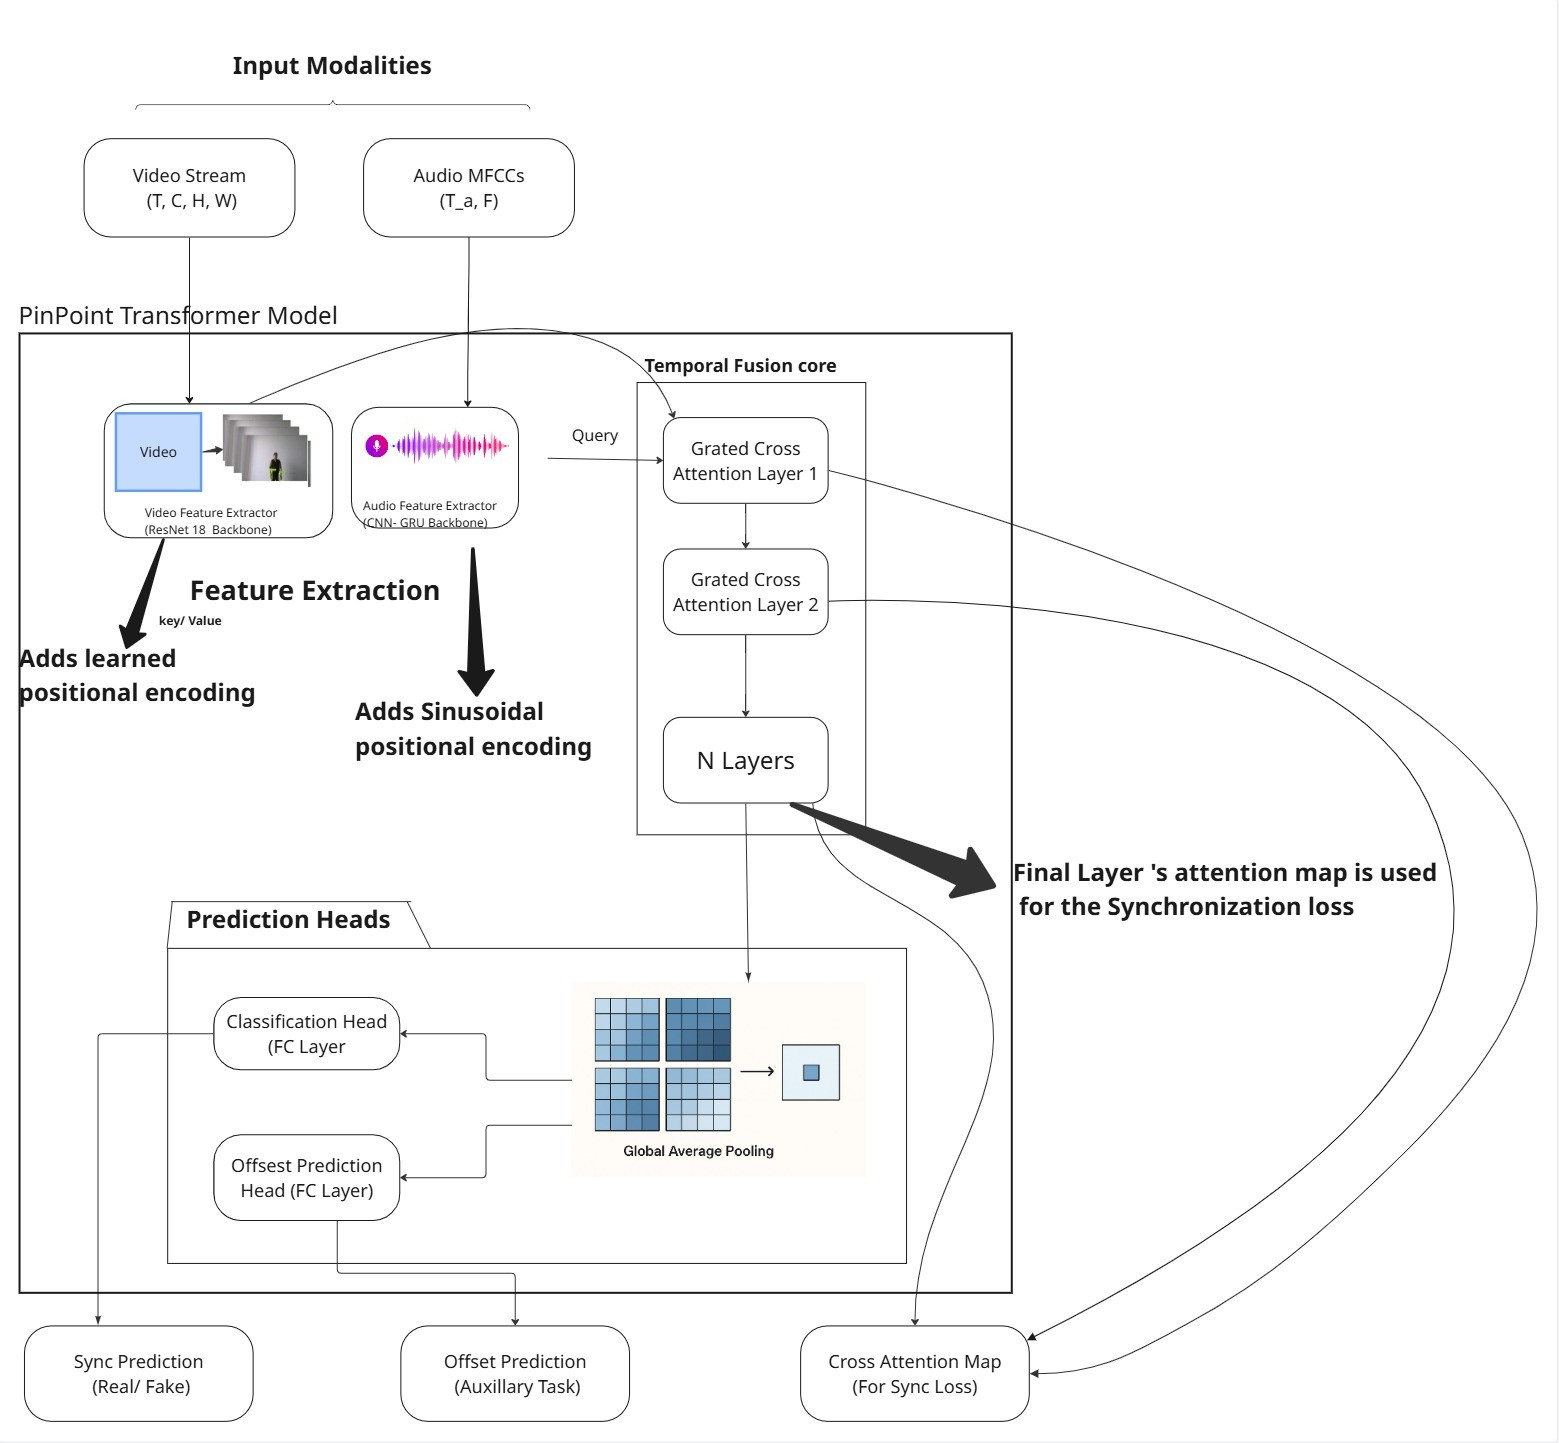
\includegraphics[width=0.86\textwidth]{image1.jpeg}
\caption{Overview of the PinPoint framework. The model receives aligned audio and video inputs, extracts modality-specific features, applies gated audio-to-video cross-attention, and trains with a curriculum that first encourages audio reliance, then synchronization learning, and finally full multimodal fusion. The synchronization loss shapes attention maps toward diagonal, smooth, and concentrated structures for aligned real samples.}
\label{fig:overview}
\end{figure}

The contributions of this paper are as follows:
\begin{enumerate}
\item We propose an audio--visual deepfake detector that uses gated cross-attention to model temporal correspondence between speech features and video frames rather than treating multimodal fusion as unconstrained feature concatenation.
\item We introduce a synchronization-aware training objective that combines soft target matching, diagonal dominance, and temporal smoothness to make cross-modal attention maps both discriminative and interpretable.
\item We train the detector with a three-stage curriculum that first masks video evidence, then emphasizes synchronization, and finally optimizes full multimodal classification.
\item We evaluate model behavior with a multimodal explainable artificial intelligence (XAI) suite that includes local attribution, attention analysis, counterfactual perturbation, and concept activation analysis.
\item We validate the design on a unified LAV-DF and FakeAVCeleb benchmark, where PinPoint achieves 97.47\% accuracy and ablation experiments show that removing the gate, synchronization loss, or curriculum sharply reduces performance.
\end{enumerate}

The remainder of the paper is organized as follows. Section~\ref{sec:related} reviews audio--visual deepfake detection and explainable multimedia forensics. Section~\ref{sec:method} presents the PinPoint architecture and training objective. Section~\ref{sec:xai} describes the explanation protocol. Section~\ref{sec:experiments} reports the experimental setup, classification results, ablations, and explanation analysis. Section~\ref{sec:discussion} discusses implications and limitations, and Section~\ref{sec:conclusion} concludes the paper.

\section{Related work}
\label{sec:related}

\subsection{Audio--visual deepfake benchmarks and synchronization cues}
\label{subsec:benchmarks}

Multimodal deepfake detection depends on datasets that contain both acoustic and visual manipulations. FakeAVCeleb introduced a multimodal benchmark containing real videos, fake audio with real video, real audio with fake video, and jointly manipulated audio--video samples \cite{khalid2021fakeavceleb}. LAV-DF later focused on content-driven audio--visual forgery and temporal localization, making it useful for studying cases where only part of a clip is manipulated \cite{cai2022lavdf}. These datasets expose a limitation of unimodal detectors: a video can appear visually plausible while its speech and facial motion are no longer temporally consistent.

Early synchronization-aware approaches used audio--visual dissonance and lip-region dynamics to detect mismatches \cite{chugh2020notmade,haliassos2021lips}. More recent systems fuse audio and visual streams with learned multimodal representations. Multimodaltrace uses separate audio and visual representations and combines them for deepfake classification \cite{raza2023multimodaltrace}. Temporal feature prediction methods exploit the expectation that adjacent audio--visual segments should be mutually predictable in authentic videos \cite{gao2024temporal}. AVSFF models lip synchronization and reports strong performance across several multimodal datasets \cite{javed2025avsff}. These studies support the value of synchronization cues, but many methods still treat alignment as an implicit consequence of architecture rather than as a directly supervised property of the learned attention map.

\subsection{Cross-modal fusion and shortcut learning}
\label{subsec:fusion}

Modern multimodal detectors increasingly rely on cross-modal attention, distillation, and hierarchical aggregation. CAD aligns multimodal representations and uses distillation to improve video deepfake detection \cite{du2025cad}. DiMoDif models differences in machine perception across modalities for detection and localization \cite{koutlis2024dimodif}. Emerging benchmarks such as MAVOS-DD further show that detectors can lose performance under open-set language and generator shifts \cite{croitoru2025mavos}. This creates a need for training objectives that discourage brittle shortcuts and push the model toward stable cross-modal evidence.

PinPoint follows this direction but differs in the role assigned to attention. Instead of using attention only as a flexible fusion operator, PinPoint makes the final audio-to-video attention map part of the supervised target. For aligned real samples, the desired attention structure is known approximately: each audio timestep should concentrate energy near the corresponding video frame and should change smoothly over time. The synchronization loss encodes this expectation directly.

\subsection{Explainability for multimedia forensics}
\label{subsec:xai_related}

Explainability is a practical requirement for multimedia forensics because a correct label does not by itself justify a decision. Feature attribution methods such as Local Interpretable Model-agnostic Explanations (LIME), SHapley Additive exPlanations (SHAP), Integrated Gradients, Layer-wise Relevance Propagation (LRP), and Gradient-weighted Class Activation Mapping (Grad-CAM) provide different views of model evidence \cite{ribeiro2016lime,lundberg2017shap,sundararajan2017ig,bach2015lrp,selvaraju2017gradcam}. Concept-based methods such as Testing with Concept Activation Vectors (TCAV) test whether human-defined concepts influence internal representations \cite{kim2018tcav}.

Deepfake-specific XAI research has begun moving from qualitative heatmaps toward quantitative explanation evaluation. Baldassarre et al. proposed metrics for explanation smoothness, locality, and sparsity in video deepfake detectors \cite{baldassarre2022metrics}. Tsigos et al. evaluated explanation methods by measuring whether highlighted regions affect detector decisions under perturbation \cite{tsigos2024xai}. Recent work in Ain Shams Engineering Journal has also emphasized unified explainable multimodal deepfake frameworks \cite{kaya2026integrated}. PinPoint builds on this trend by evaluating not only visual saliency but also audio attribution, attention structure, counterfactual sensitivity, and concept-level response to lip-sync error.

\section{Materials and methods}
\label{sec:method}

\subsection{Problem formulation and inputs}
\label{subsec:formulation}

Given a video segment $V$ and its corresponding audio representation $A$, the task is to predict a binary label $y \in \{0,1\}$, where $0$ denotes real and $1$ denotes fake. Each video sample is represented by 30 RGB frames resized to $128 \times 128$ and normalized with ImageNet mean and standard deviation. Each audio sample is represented as a time sequence of 13-dimensional MFCC features. The model outputs a fake logit, an auxiliary audio--video offset prediction, and the final audio-to-video attention map used for synchronization analysis.

\subsection{Dataset construction and preprocessing}
\label{subsec:data}

The experiments use a unified preprocessed benchmark built from LAV-DF and FakeAVCeleb. The dataset keeps the available train, validation, and test split metadata instead of re-splitting samples locally. Table~\ref{tab:splits} reports the resulting split sizes and class balance. The test split contains 26,097 samples, with 6,906 real and 19,191 fake samples.

\begin{table}[H]
\caption{Unified benchmark split sizes and class balance.}
\label{tab:splits}
\centering
\begin{tabular}{lrrrr}
\toprule
Split & Total & Real & Fake & Real/Fake ratio \\
\midrule
Train & 78,703 & 21,254 & 57,449 & 0.37 \\
Validation & 31,501 & 8,271 & 23,230 & 0.36 \\
Test & 26,097 & 6,906 & 19,191 & 0.36 \\
\bottomrule
\end{tabular}
\end{table}

During training, video augmentations include JPEG compression, random noise, Gaussian blur, low-resolution resizing artifacts, color jitter, and random erasing. These augmentations are intended to reduce dependence on low-level generator artifacts. A modality dropout probability of 0.15 randomly drops either audio or video features for a sample during training, forcing the model to preserve useful evidence from both streams. For real training samples, artificial audio offsets are inserted with probability 0.5 over a maximum offset range of five video frames. These offset labels supervise the auxiliary offset prediction head.

\subsection{PinPoint architecture}
\label{subsec:architecture}

PinPoint contains a visual encoder, an audio encoder, stacked gated cross-attention blocks, and two prediction heads. The visual encoder is an ImageNet-pretrained ResNet-18 \cite{he2016resnet}. To support gradient-based explanation methods, all in-place rectified linear unit operations and residual additions are patched into non-in-place operations. The final convolutional features are adaptively pooled and projected to a 256-dimensional frame embedding. Early ResNet layers are frozen during training.

The audio encoder contains two one-dimensional convolution layers followed by layer normalization and a Gated Recurrent Unit (GRU). The convolution layers map 13 MFCC channels to 64 and then 128 channels using kernel size 3 and padding 1. The GRU maps the sequence to the same 256-dimensional embedding space as the video stream. Video embeddings use learned positional encodings, while audio embeddings use sinusoidal positional encodings.

Fusion uses three gated cross-attention blocks. In each block, audio embeddings act as queries and video embeddings act as keys and values. The resulting attention map therefore answers a temporally meaningful question: for each audio timestep, which video frames support the current representation? Figure~\ref{fig:gated} illustrates the block. After cross-attention, a sigmoid gate filters the attended audio representation. The gated representation then passes through audio self-attention and a feed-forward network with a hidden dimension of $4d$, where $d=256$.

\begin{figure}[H]
\centering
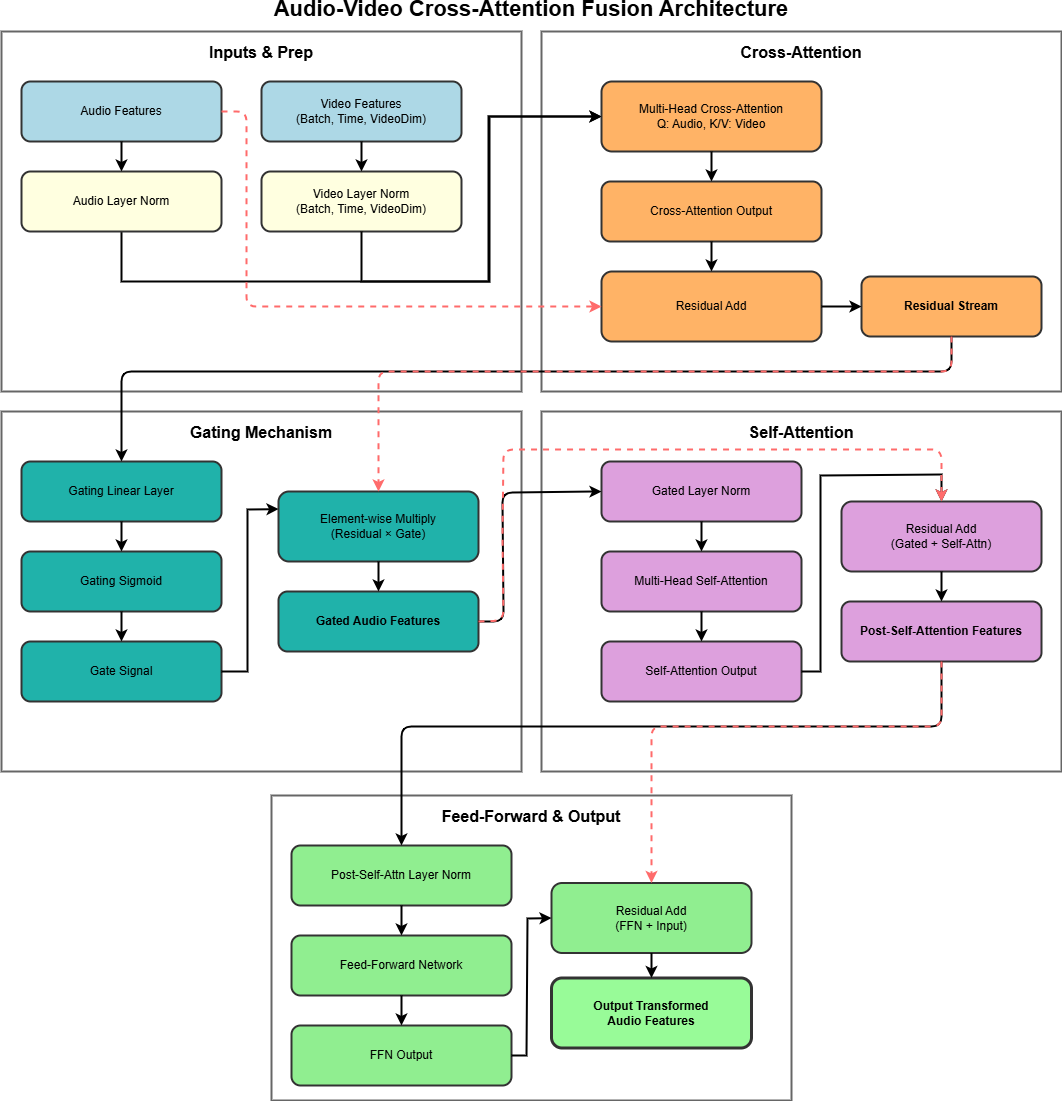
\includegraphics[width=0.72\textwidth]{image2.png}
\caption{Gated cross-attention block. Audio features query video features, producing an audio-to-video attention map. A learned sigmoid gate filters the attended representation before self-attention and feed-forward refinement.}
\label{fig:gated}
\end{figure}

The final audio sequence is mean-pooled and passed to two heads. The classification head predicts the fake logit. The auxiliary offset head predicts one of $2M+1$ offset classes, where $M=5$ is the maximum frame offset. This auxiliary task gives the model an explicit training signal for temporal misalignment on real samples.

\subsection{Synchronization-aware loss}
\label{subsec:sync_loss}

The synchronization loss shapes the final cross-attention map for real samples whose audio and video are aligned. Let $\mathbf{A}\in\mathbb{R}^{N \times M}$ denote the attention map between $N$ audio timesteps and $M$ video frames. The loss combines direct target matching, diagonal dominance, and temporal smoothness:

\begin{equation}
\mathcal{L}_{sync} =
\lambda_{mse}\mathcal{L}_{mse}
+ \lambda_{diag}\mathcal{L}_{diag}
+ \lambda_{smooth}\mathcal{L}_{smooth},
\label{eq:sync_total}
\end{equation}

where $\lambda_{mse}=1.0$, $\lambda_{diag}=0.5$, and $\lambda_{smooth}=0.2$. The first term matches the attention map to a soft diagonal target:

\begin{equation}
\mathcal{L}_{mse}
= \frac{1}{NM}\sum_{i=1}^{N}\sum_{j=1}^{M}(A_{ij}-T_{ij})^2 .
\label{eq:mse}
\end{equation}

The target $T_{ij}$ is a normalized Gaussian band around the expected corresponding video frame:

\begin{equation}
T_{ij} =
\frac{\exp\left(-(j-c_i)^2/(2\sigma^2)\right)}
{\sum_{m=1}^{M}\exp\left(-(m-c_i)^2/(2\sigma^2)\right)} ,
\label{eq:target}
\end{equation}

where $c_i=\lfloor i/r \rfloor$, $r=2$ MFCC timesteps per video frame, and $\sigma=2$. The second term penalizes attention energy outside a diagonal band of width $b=2$:

\begin{equation}
\mathcal{L}_{diag}
= 1 -
\frac{\sum_{i=1}^{N}\sum_{|j-c_i|\leq b}A_{ij}}
{\sum_{i=1}^{N}\sum_{j=1}^{M}A_{ij}} .
\label{eq:diag}
\end{equation}

The third term discourages abrupt changes across neighboring audio timesteps and video frames:

\begin{equation}
\mathcal{L}_{smooth}
= \frac{1}{N-1}\sum_{i=1}^{N-1}\sum_{j=1}^{M}(A_{ij}-A_{i+1,j})^2
+ \frac{1}{M-1}\sum_{i=1}^{N}\sum_{j=1}^{M-1}(A_{ij}-A_{i,j+1})^2 .
\label{eq:smooth}
\end{equation}

The loss is applied only to aligned real samples. Fake samples and artificially offset real samples do not have a diagonal synchronization target, so they are excluded from this term.

\subsection{Training objective and curriculum}
\label{subsec:training}

The total loss combines binary classification, auxiliary offset prediction, and synchronization supervision:

\begin{equation}
\mathcal{L}_{total}
= W_{class}\mathcal{L}_{class}
+ W_{offset}\mathcal{L}_{offset}
+ W_{sync}\mathcal{L}_{sync},
\label{eq:total}
\end{equation}

where $W_{class}=1.0$, $W_{offset}=0.5$, and $W_{sync}=3.0$. The classification term uses binary cross-entropy with logits and a positive-class weight computed from the real/fake composition of the training split. The offset term uses cross-entropy over 11 offset classes and is applied only to real samples.

Training follows a three-stage curriculum. In Phase 1, covering the first two epochs, 50--80\% of video frames are randomly masked to force the model to learn useful audio evidence. In Phase 2, covering the next three epochs, synchronization learning receives emphasis and the offset loss is down-weighted by a factor of 0.1. In Phase 3, covering the remaining ten epochs, the model trains with full multimodal evidence and the complete composite objective. Table~\ref{tab:hyperparameters} summarizes the main training settings.

\begin{table}[H]
\caption{Key implementation settings for PinPoint.}
\label{tab:hyperparameters}
\centering
\small
\setlength{\tabcolsep}{4pt}
\begin{tabularx}{\textwidth}{l>{\raggedright\arraybackslash}X}
\toprule
Parameter & Value \\
\midrule
Video input & 30 frames, $128 \times 128$ RGB \\
Audio input & 13 MFCC coefficients per timestep \\
Visual encoder & ImageNet-pretrained ResNet-18 \\
Audio encoder & Conv1D(64), Conv1D(128), LayerNorm, GRU(256) \\
Embedding dimension & 256 \\
Cross-attention heads / layers & 8 / 3 \\
Dropout & 0.1 \\
Batch size / epochs & 4 / 15 \\
Optimizer & AdamW \\
Learning rate / weight decay & $1\times10^{-4}$ / $1\times10^{-4}$ \\
Learning-rate schedule & Cosine annealing \\
Gradient clipping & 1.0 maximum norm \\
Modality dropout & 0.15 \\
Maximum offset & 5 video frames \\
Offset probability & 0.5 for real training samples \\
\bottomrule
\end{tabularx}
\end{table}

\section{Explainable AI evaluation protocol}
\label{sec:xai}

PinPoint is evaluated with complementary explanation tools because no single explanation method is sufficient for a multimodal forensic model. The XAI protocol tests four forms of evidence: local feature attribution, temporal attention structure, counterfactual sensitivity, and concept-level response.

\subsection{Attribution and attention methods}
\label{subsec:attribution}

Integrated Gradients and LRP produce gradient- and relevance-based attribution maps over video frames and MFCC features. SHAP estimates feature contribution relative to a small background set, and LIME builds local surrogate explanations for both modalities. Attention analysis visualizes the final cross-attention map and attention rollout across stacked attention layers. These methods provide complementary checks: agreement between independent attribution methods increases confidence that the highlighted evidence is not an artifact of a single explainer.

\begin{figure}[H]
\centering
\begin{subfigure}[b]{0.32\textwidth}
\centering
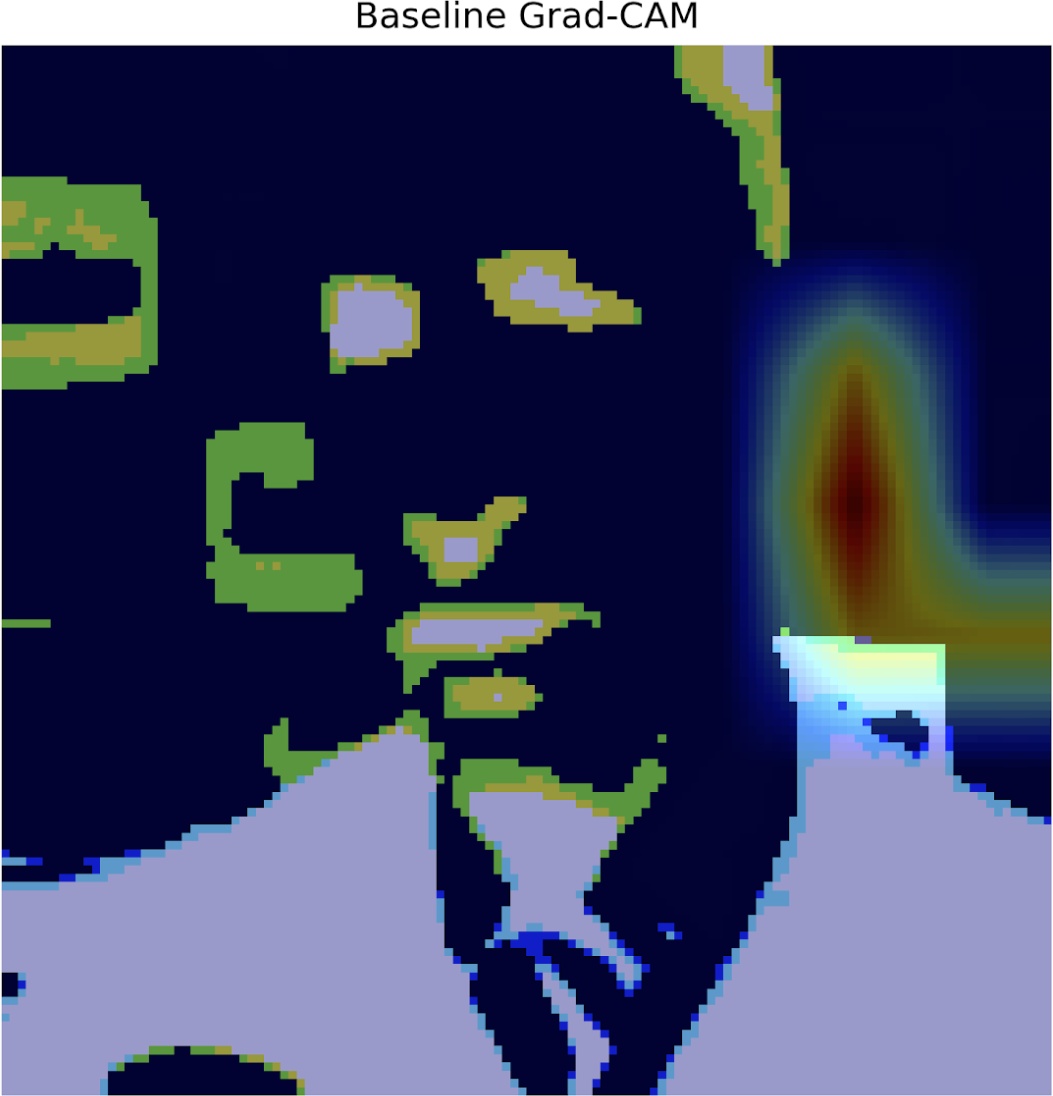
\includegraphics[width=\textwidth]{image3.png}
\caption{Grad-CAM}
\end{subfigure}
\hfill
\begin{subfigure}[b]{0.32\textwidth}
\centering
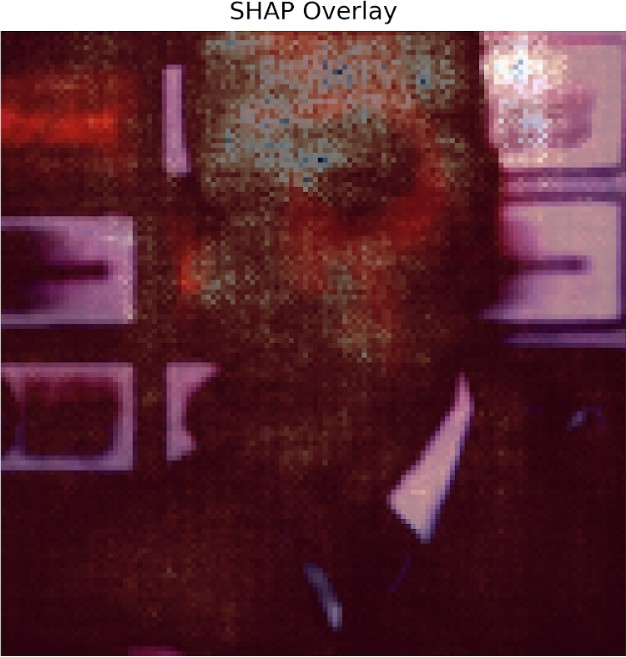
\includegraphics[width=\textwidth]{image4.jpeg}
\caption{SHAP}
\end{subfigure}
\hfill
\begin{subfigure}[b]{0.32\textwidth}
\centering
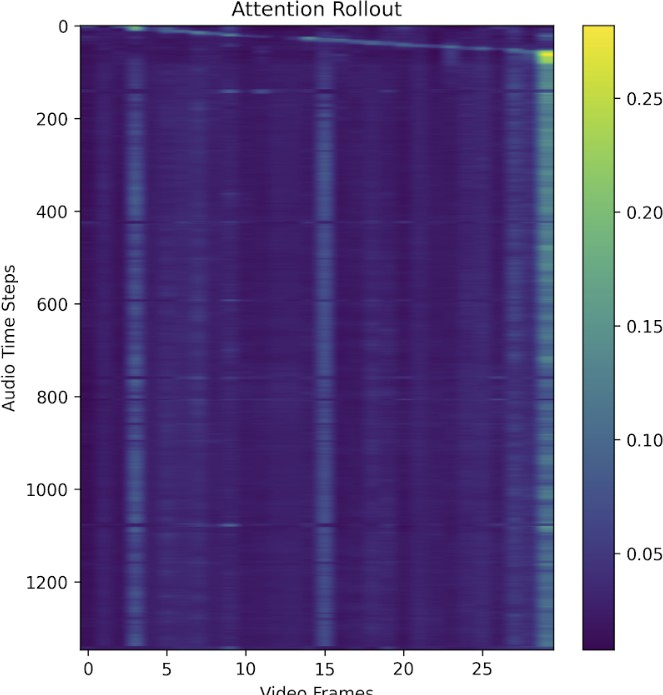
\includegraphics[width=\textwidth]{image5.jpeg}
\caption{Attention rollout}
\end{subfigure}
\caption{Example multimodal explanations for a fake sample. Grad-CAM and SHAP highlight visual evidence around the face and mouth region, while attention rollout exposes the temporal structure used during audio--visual fusion.}
\label{fig:xai_suite}
\end{figure}

\subsection{Counterfactual and concept analysis}
\label{subsec:counterfactual_tcav}

Counterfactual analysis searches for small audio and video perturbations that change the predicted class. This provides a causal stress test: if changing the highlighted visual or acoustic evidence flips the decision, the explanation is more informative than a static heatmap alone. TCAV evaluates whether the model is sensitive to a human-defined lip-sync error concept by training concept activation vectors at selected internal layers and measuring whether movement in that concept direction changes the fake-class output.

\subsection{Quantitative explanation metrics}
\label{subsec:xai_metrics}

The quantitative analysis reports sparsity and inter-technique consistency. Sparsity is measured with the Gini index:

\begin{equation}
G = \frac{\sum_{i=1}^{n}(2i-n-1)x_i}{n\sum_{i=1}^{n}x_i},
\label{eq:gini}
\end{equation}

where $x_i$ are sorted attribution values. Higher values indicate more concentrated attribution. Inter-technique consistency is measured with Spearman rank correlation between flattened attribution maps from different explanation methods:

\begin{equation}
\rho = 1 - \frac{6\sum d_i^2}{n(n^2-1)},
\label{eq:spearman}
\end{equation}

where $d_i$ is the rank difference for feature $i$. Consistency is important because high sparsity alone is not necessarily desirable; a sparse explanation can still focus on unstable or irrelevant evidence.

\section{Experiments and results}
\label{sec:experiments}

\subsection{Main classification performance}
\label{subsec:main_results}

Table~\ref{tab:main_performance} reports the full PinPoint model on the unified test split. The model correctly classifies 25,436 of 26,097 samples, giving 97.47\% accuracy. Fake-class F1 reaches 0.9825, and real-class recall reaches 0.98. The high real-class recall is important because a forensic detector should avoid incorrectly accusing authentic content whenever possible.

\begin{table}[H]
\caption{PinPoint performance on the unified LAV-DF and FakeAVCeleb test split.}
\label{tab:main_performance}
\centering
\begin{tabular}{lrrrr}
\toprule
Class / aggregate & Precision & Recall & F1-score & Support \\
\midrule
Real & 0.93 & 0.98 & 0.9535 & 6,906 \\
Fake & 0.99 & 0.97 & 0.9825 & 19,191 \\
\midrule
Macro average & 0.96 & 0.98 & 0.9680 & 26,097 \\
Weighted average & 0.98 & 0.97 & 0.9700 & 26,097 \\
Accuracy & -- & -- & 97.47\% & 26,097 \\
\bottomrule
\end{tabular}
\end{table}

The confusion matrix in Table~\ref{tab:confusion} shows that most errors are fake samples predicted as real. This pattern is preferable to an uncontrolled false-positive tendency, but it also indicates that future work should test more difficult manipulation families and calibrate decision thresholds for the intended forensic setting.

\begin{table}[H]
\caption{Confusion matrix for the full PinPoint model on the unified test split.}
\label{tab:confusion}
\centering
\begin{tabular}{lrr}
\toprule
Ground truth & Predicted real & Predicted fake \\
\midrule
Real & 6,767 & 139 \\
Fake & 522 & 18,669 \\
\bottomrule
\end{tabular}
\end{table}

Table~\ref{tab:contextual_comparison} places the result beside representative audio--visual detectors. This table should not be read as a strict leaderboard because the compared papers use different datasets, splits, and evaluation protocols. Its purpose is to contextualize the performance range of recent multimodal methods while keeping PinPoint's primary evidence in the unified benchmark and ablation study.

\begin{table}[H]
\caption{Contextual comparison with representative audio--visual deepfake detectors. Metrics are not directly comparable across rows because datasets and protocols differ.}
\label{tab:contextual_comparison}
\centering
\scriptsize
\setlength{\tabcolsep}{3pt}
\begin{tabularx}{\textwidth}{p{3.3cm}p{2.6cm}rrrr}
\toprule
Method & Dataset(s) & Accuracy & Precision & Recall & F1-score \\
\midrule
PinPoint & Unified benchmark & 97.47\% & 0.98 & 0.97 & 0.97 \\
AVSFF \cite{javed2025avsff} & FakeAVCeleb & 99.73\% & 0.9971 & 0.9944 & 0.9907 \\
AVSFF \cite{javed2025avsff} & LAV-DF & 97.86\% & -- & -- & -- \\
Multimodaltrace \cite{raza2023multimodaltrace} & FakeAVCeleb & 92.9\% & -- & -- & 0.945 \\
TFP \cite{gao2024temporal} & FakeAVCeleb & 84.33\% & -- & -- & -- \\
\bottomrule
\end{tabularx}
\end{table}

\subsection{Ablation study}
\label{subsec:ablations}

The ablation study isolates the gate, synchronization loss, and curriculum while keeping the unified evaluation protocol fixed. Table~\ref{tab:ablation} shows that each component contributes to performance. Removing the gate causes the largest degradation, reducing accuracy from 97.47\% to 58.35\%. Removing the synchronization loss reduces accuracy to 75.47\%, and removing the curriculum reduces accuracy to 81.44\%.

\begin{table}[H]
\caption{Ablation study on the unified test split. Each variant removes one component from the full model.}
\label{tab:ablation}
\centering
\small
\setlength{\tabcolsep}{3pt}
\begin{tabular}{lrrrrr}
\toprule
Variant & Epochs & Accuracy & Fake F1 & Fake precision & Fake recall \\
\midrule
Full PinPoint & 15 & 97.47\% & 0.9825 & 0.99 & 0.97 \\
No synchronization loss & 15 & 75.47\% & 0.8067 & 0.95 & 0.70 \\
No gate & 15 & 58.35\% & 0.6115 & 0.97 & 0.45 \\
No curriculum & 15 & 81.44\% & 0.8639 & 0.94 & 0.80 \\
\bottomrule
\end{tabular}
\end{table}

The gate is therefore not a minor architectural embellishment. It controls how much cross-modal evidence enters the refined audio representation, and removing it leaves the model with standard cross-attention that performs poorly on fake recall. The synchronization loss is also essential: without direct alignment supervision, the model retains high fake precision but misses many manipulated samples. The curriculum result shows that training order changes the learned decision behavior, not merely the speed of convergence.

\begin{figure}[H]
\centering
\begin{subfigure}[b]{0.48\textwidth}
\centering
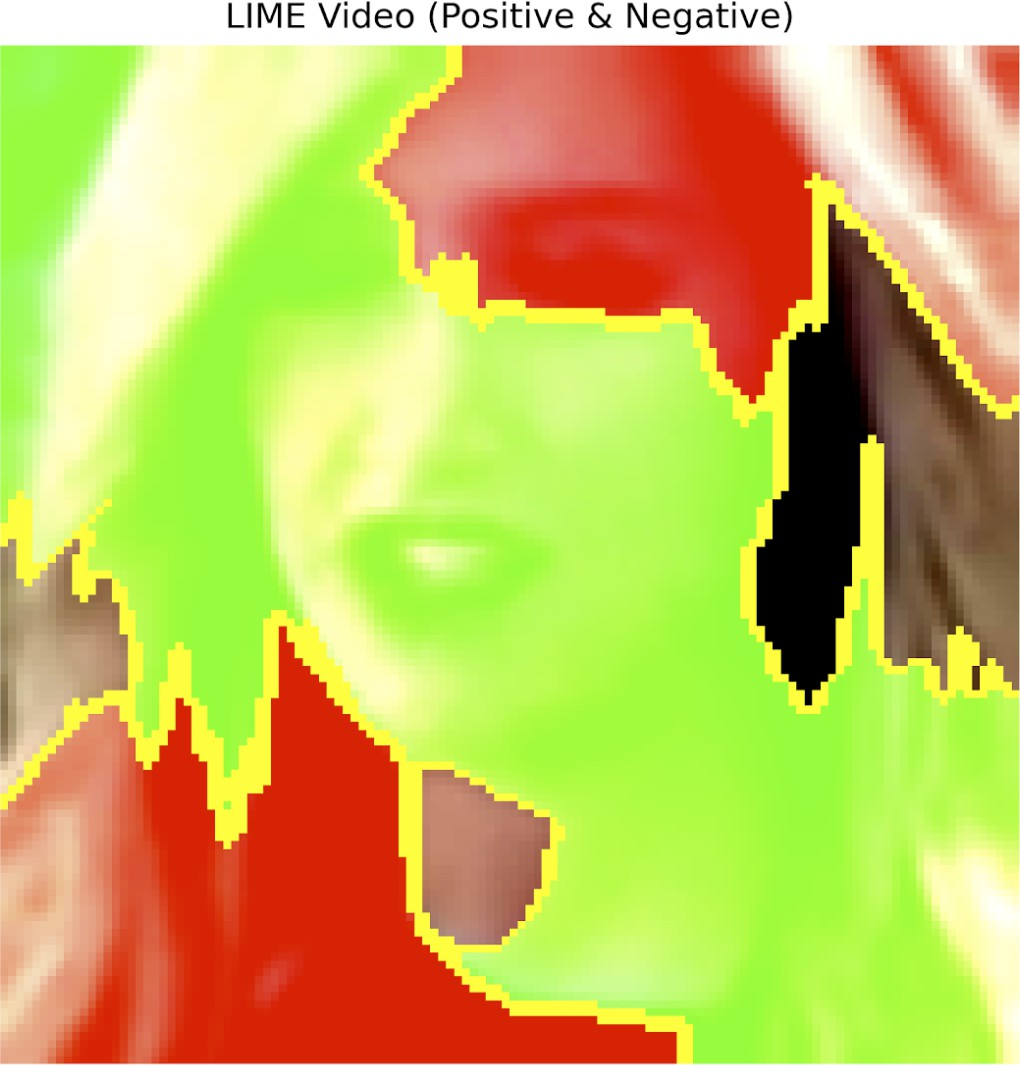
\includegraphics[width=\textwidth]{image6.jpeg}
\caption{Full PinPoint}
\end{subfigure}
\hfill
\begin{subfigure}[b]{0.48\textwidth}
\centering
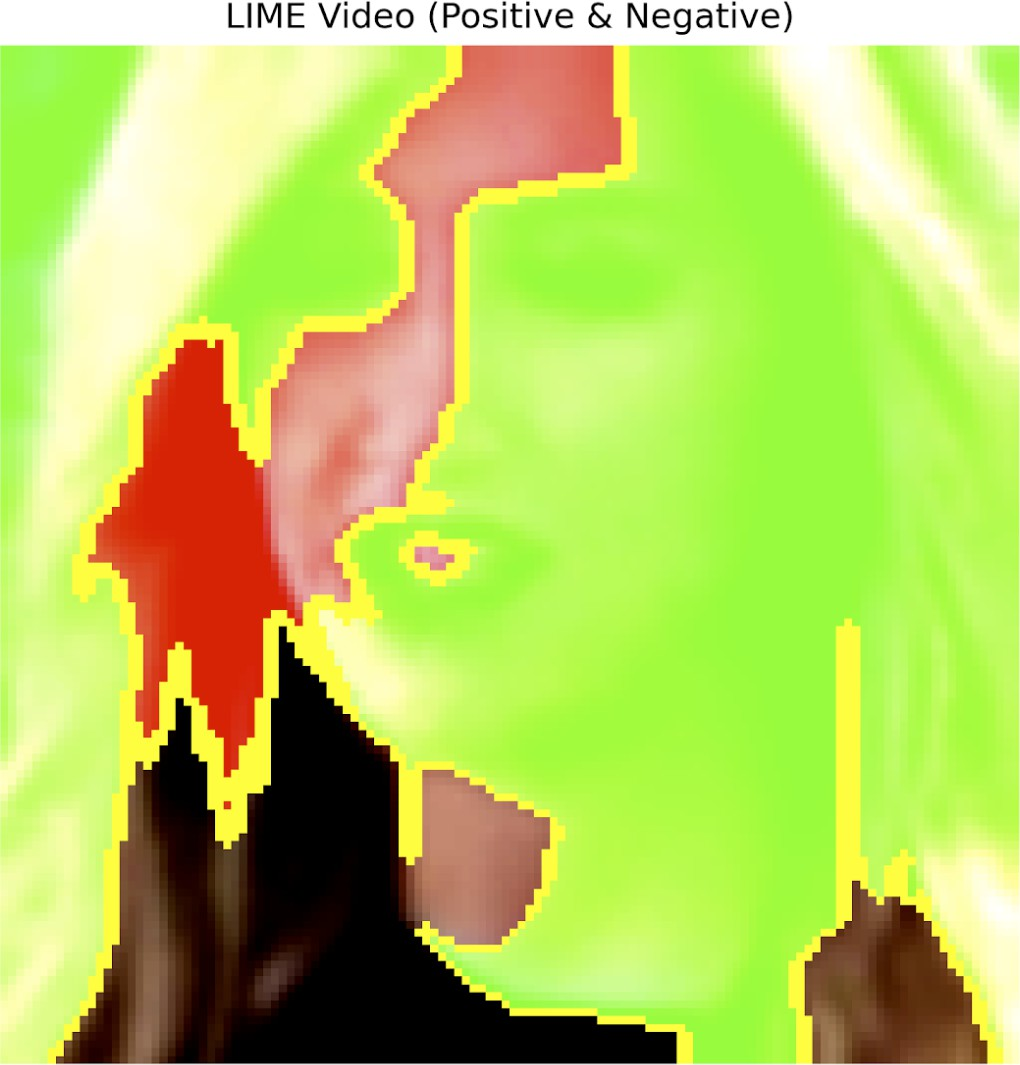
\includegraphics[width=\textwidth]{image7.jpeg}
\caption{No synchronization loss}
\end{subfigure}

\begin{subfigure}[b]{0.48\textwidth}
\centering
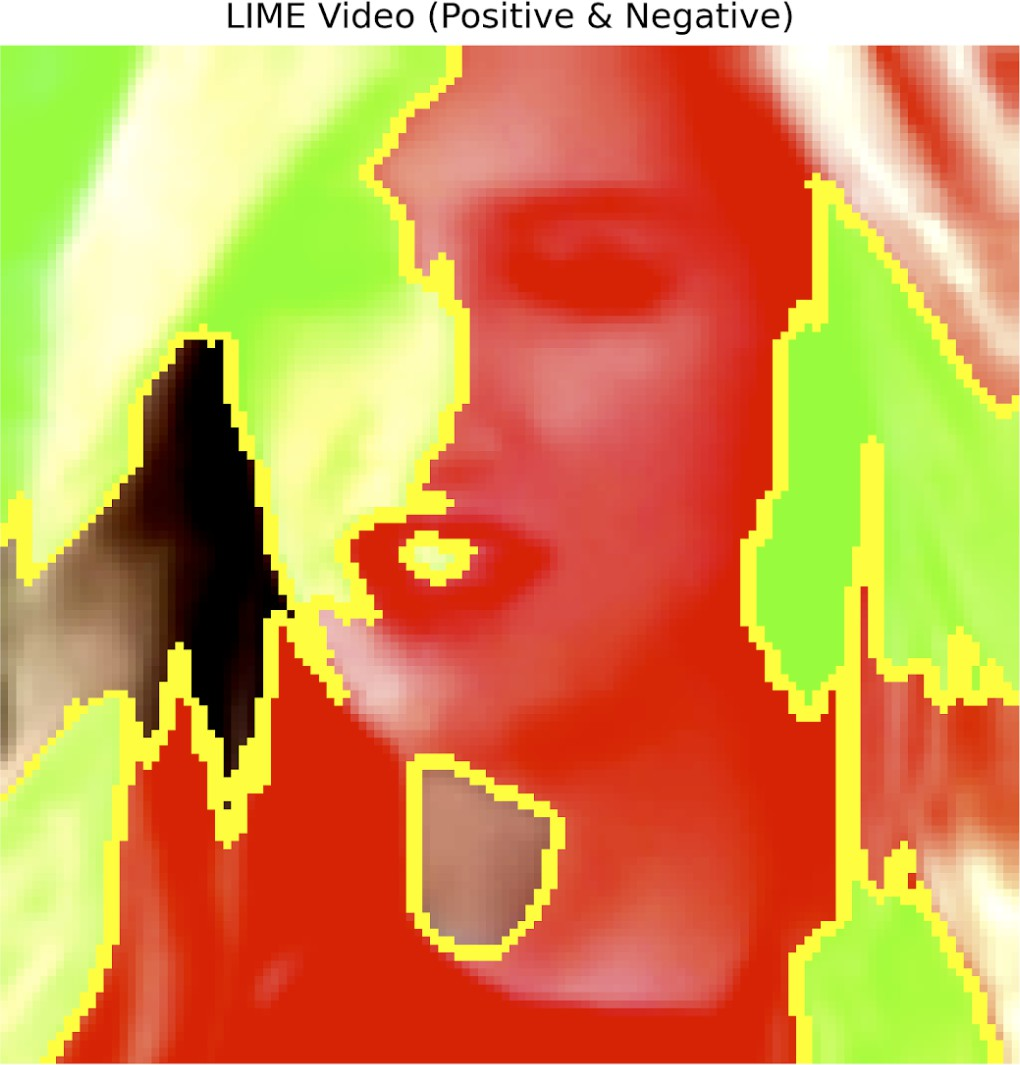
\includegraphics[width=\textwidth]{image8.jpeg}
\caption{No gate}
\end{subfigure}
\hfill
\begin{subfigure}[b]{0.48\textwidth}
\centering
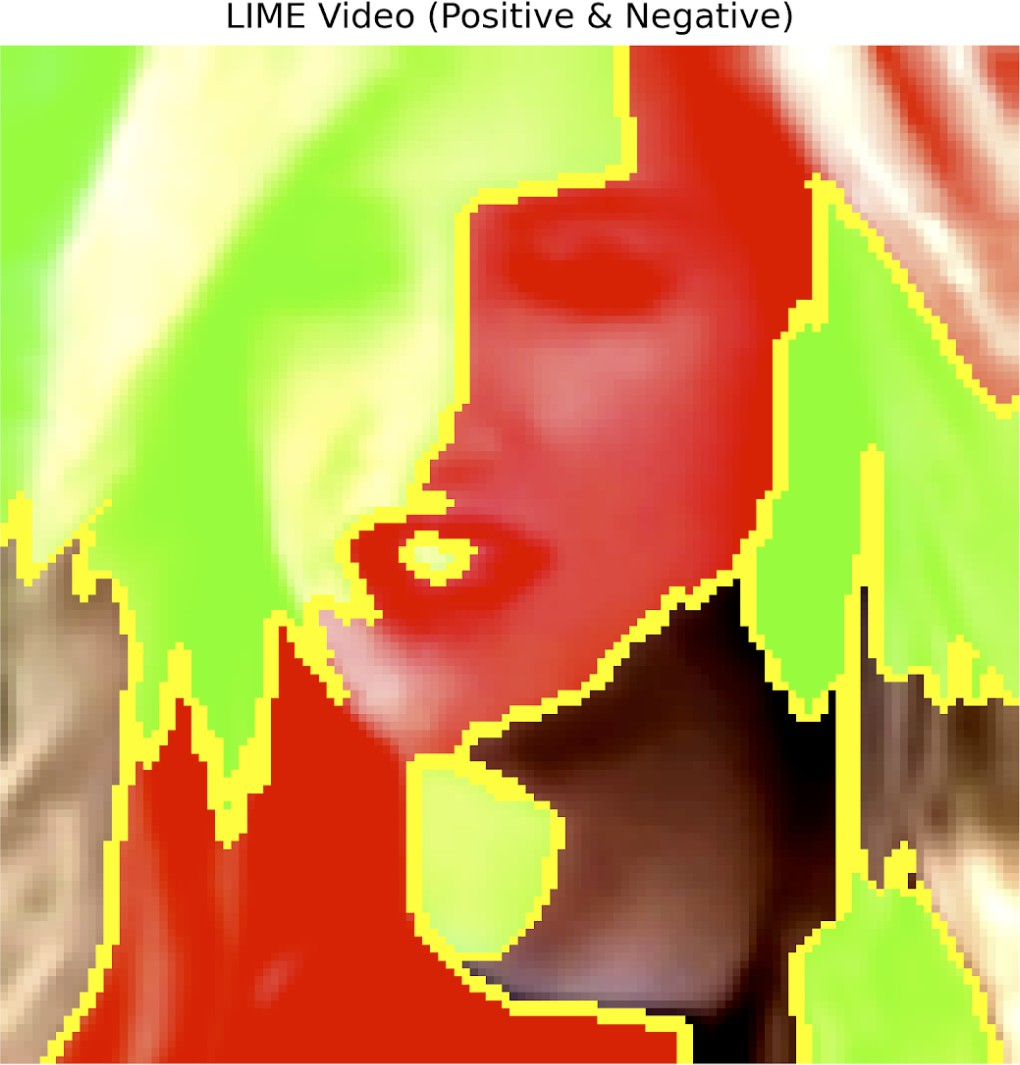
\includegraphics[width=\textwidth]{image9.jpeg}
\caption{No curriculum}
\end{subfigure}
\caption{LIME visualizations across model variants. The full model concentrates evidence more coherently around the mouth and face region, while ablated variants produce less stable or more diffuse visual explanations.}
\label{fig:lime_ablation}
\end{figure}

\subsection{Quantitative explanation results}
\label{subsec:quant_xai}

Table~\ref{tab:xai_metrics} reports explanation metrics for the full model and ablations. PinPoint produces moderate video sparsity, strong audio sparsity, and the highest inter-technique consistency among the evaluated variants. The consistency result is the most important part of the table: multiple explanation methods agree more strongly for the full model, suggesting that the model's evidence is more stable under different attribution lenses.

\begin{table}[H]
\caption{Quantitative XAI metrics across model variants. Higher consistency indicates stronger agreement between explanation methods.}
\label{tab:xai_metrics}
\centering
\small
\setlength{\tabcolsep}{4pt}
\begin{tabular}{lrrr}
\toprule
Model & Video Gini & Audio Gini & Consistency (Spearman) \\
\midrule
Full PinPoint & 0.631 & 0.928 & 0.514 \\
No curriculum & 0.803 & 0.919 & 0.450 \\
No gate & 0.753 & 0.760 & 0.372 \\
No synchronization loss & 0.708 & 0.883 & 0.436 \\
\bottomrule
\end{tabular}
\end{table}

Higher Gini values in the ablated models should not be interpreted as automatically better. A sparse explanation can be unhelpful if it focuses on unstable evidence. The full model's combination of concentrated audio attribution and higher inter-technique consistency better matches the forensic requirement: explanations should be both localized and repeatable.

\subsection{Case studies}
\label{subsec:case_studies}

Figure~\ref{fig:attention_maps} compares attention maps for real and fake samples. The real sample shows a stronger diagonal pattern, indicating that audio timesteps attend to temporally corresponding video frames. The fake sample produces a more diffuse map, consistent with weaker audio--visual synchrony. This is the intended behavior of the synchronization loss: the attention map becomes an interpretable object rather than only a hidden fusion mechanism.

\begin{figure}[H]
\centering
\begin{subfigure}[b]{0.46\textwidth}
\centering
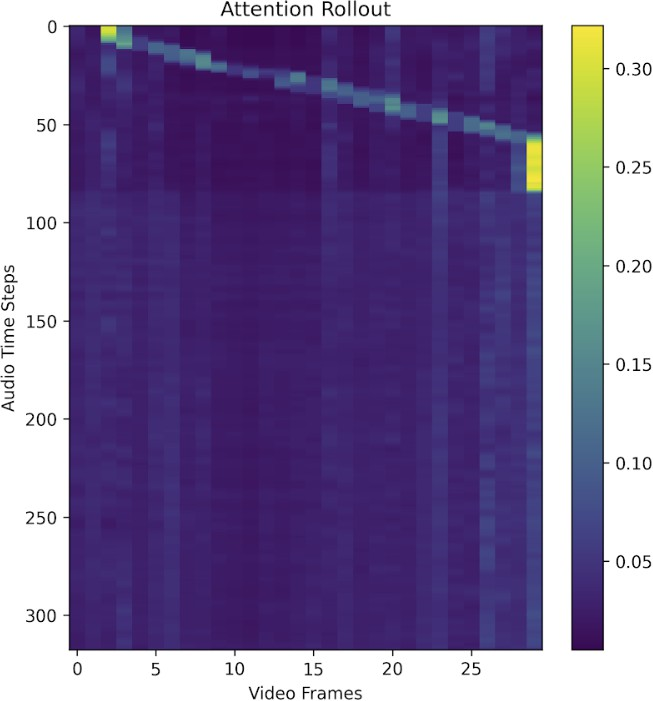
\includegraphics[width=0.72\textwidth]{image10.jpeg}
\caption{Real sample}
\end{subfigure}
\hfill
\begin{subfigure}[b]{0.46\textwidth}
\centering
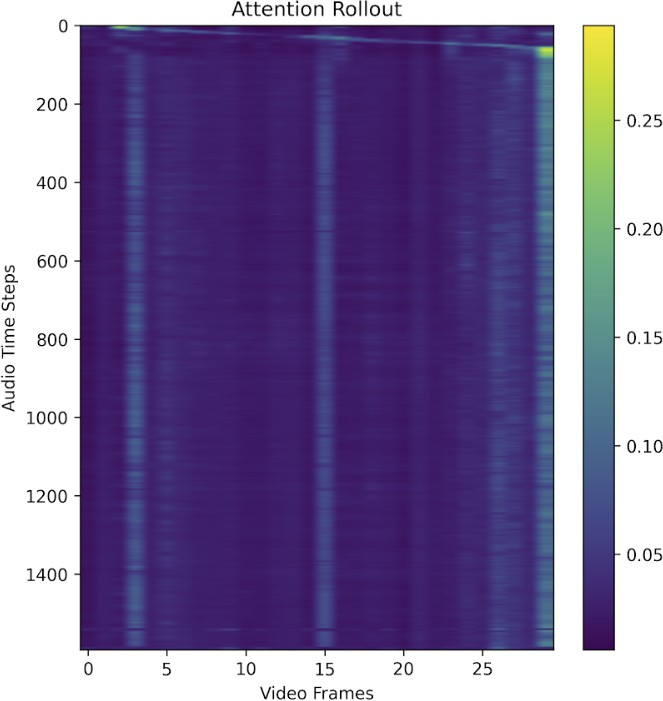
\includegraphics[width=0.72\textwidth]{image11.jpeg}
\caption{Fake sample}
\end{subfigure}
\caption{Cross-attention maps for representative real and fake samples. Real samples exhibit stronger diagonal alignment, while fake samples show more diffuse attention, indicating weaker audio--visual correspondence.}
\label{fig:attention_maps}
\end{figure}

Figure~\ref{fig:attribution_case} shows visual attribution on a fake sample. Grad-CAM emphasizes the mouth and lower-face region, while SHAP provides a complementary attribution view. These attributions agree with the synchronization framing because lip motion and mouth-region evidence are expected to carry much of the audio--visual mismatch signal.

\begin{figure}[H]
\centering
\begin{subfigure}[b]{0.32\textwidth}
\centering
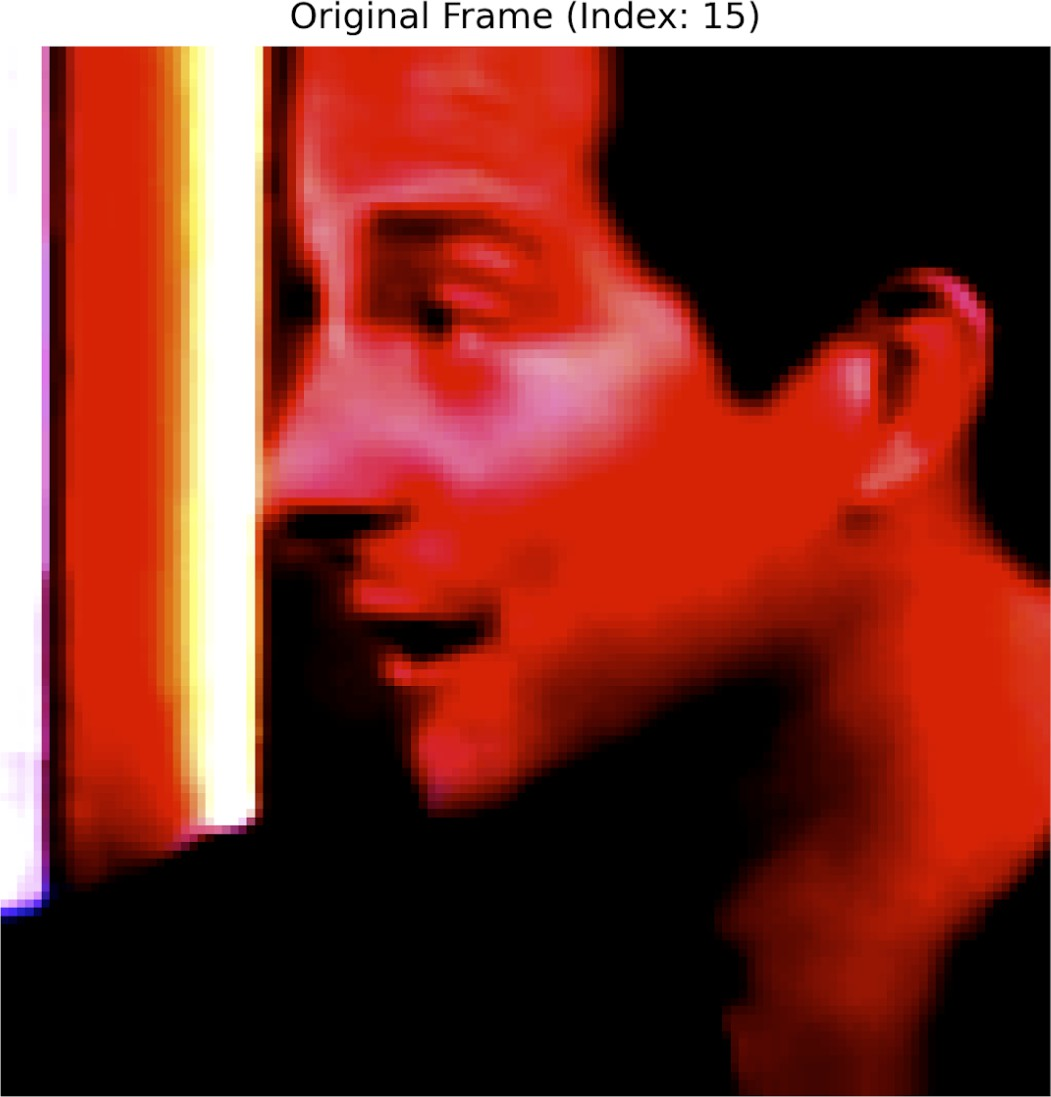
\includegraphics[width=\textwidth]{image12.jpeg}
\caption{Original frame}
\end{subfigure}
\hfill
\begin{subfigure}[b]{0.32\textwidth}
\centering
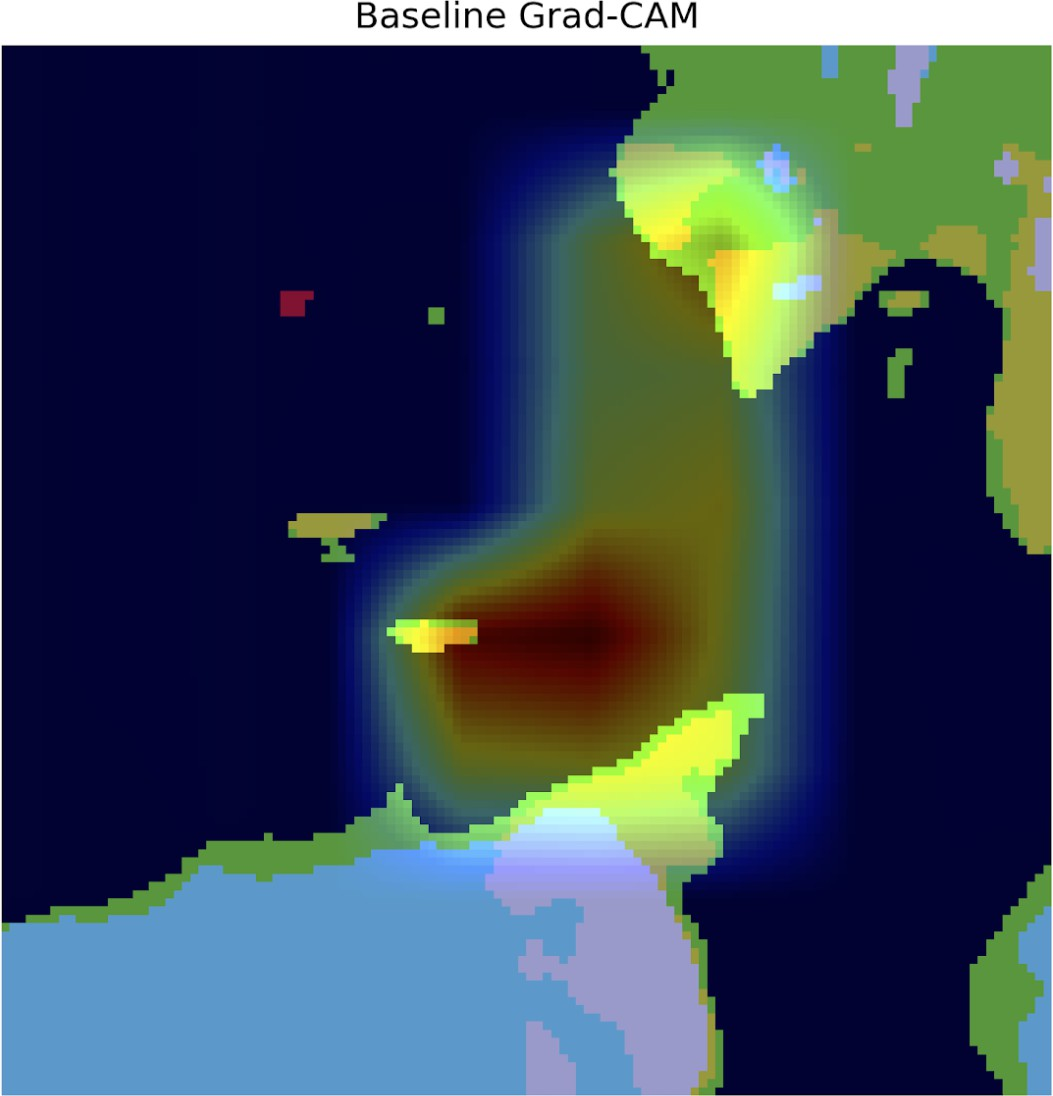
\includegraphics[width=\textwidth]{image13.jpeg}
\caption{Grad-CAM}
\end{subfigure}
\hfill
\begin{subfigure}[b]{0.32\textwidth}
\centering
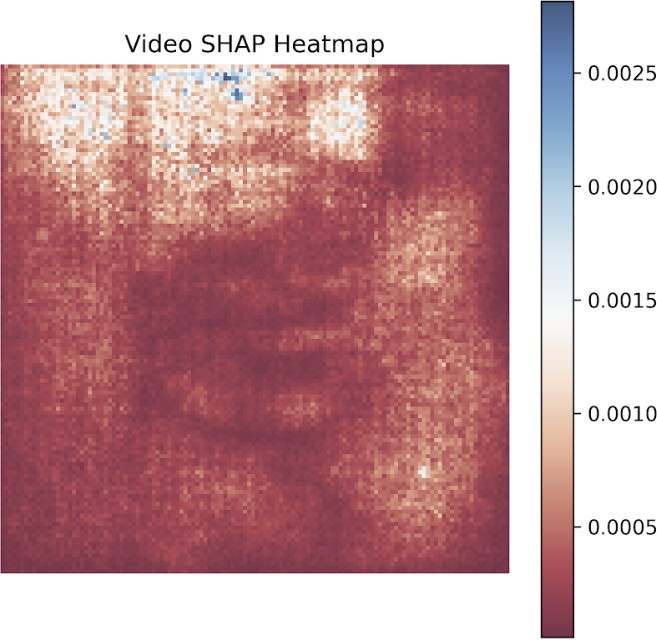
\includegraphics[width=\textwidth]{image14.jpeg}
\caption{SHAP}
\end{subfigure}
\caption{Attribution case study. Visual explanation methods identify face and mouth-region evidence that supports the fake prediction, complementing the temporal evidence from cross-attention.}
\label{fig:attribution_case}
\end{figure}

Counterfactual analysis tests whether changing the highlighted evidence can alter the prediction. Figure~\ref{fig:counterfactual} shows a perturbation that changes a fake prediction toward real. The difference map localizes the visual evidence responsible for the decision shift, providing a stronger check than a purely descriptive saliency map.

\begin{figure}[H]
\centering
\begin{subfigure}[b]{0.32\textwidth}
\centering
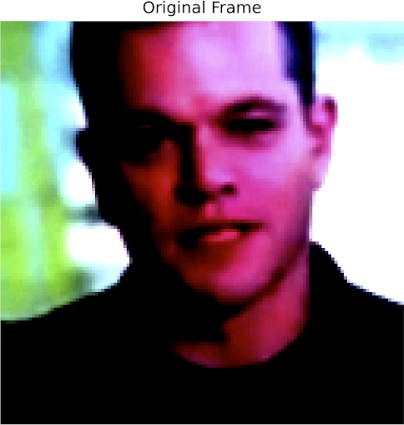
\includegraphics[width=\textwidth]{image16.jpeg}
\caption{Original frame}
\end{subfigure}
\hfill
\begin{subfigure}[b]{0.32\textwidth}
\centering
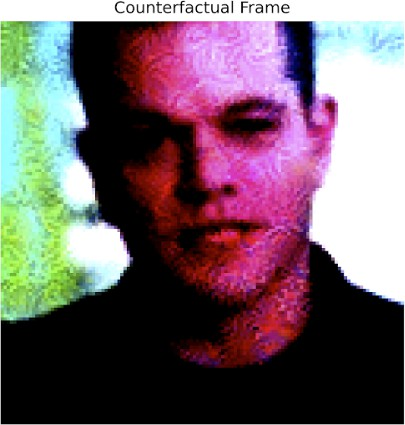
\includegraphics[width=\textwidth]{image17.jpeg}
\caption{Counterfactual frame}
\end{subfigure}
\hfill
\begin{subfigure}[b]{0.32\textwidth}
\centering
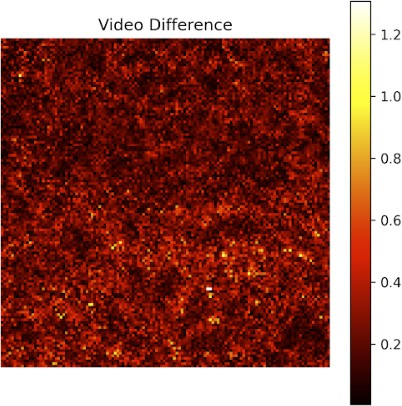
\includegraphics[width=\textwidth]{image15.jpeg}
\caption{Difference map}
\end{subfigure}
\caption{Counterfactual explanation. A small perturbation changes the model decision, and the difference map localizes the visual evidence most responsible for the decision shift.}
\label{fig:counterfactual}
\end{figure}

The TCAV analysis further tests concept-level behavior. Figure~\ref{fig:tcav} shows high sensitivity to the lip-sync error concept at the gated attention layer and classification head. These results support the claim that synchronization information influences both the internal representation and the final decision.

\begin{figure}[H]
\centering
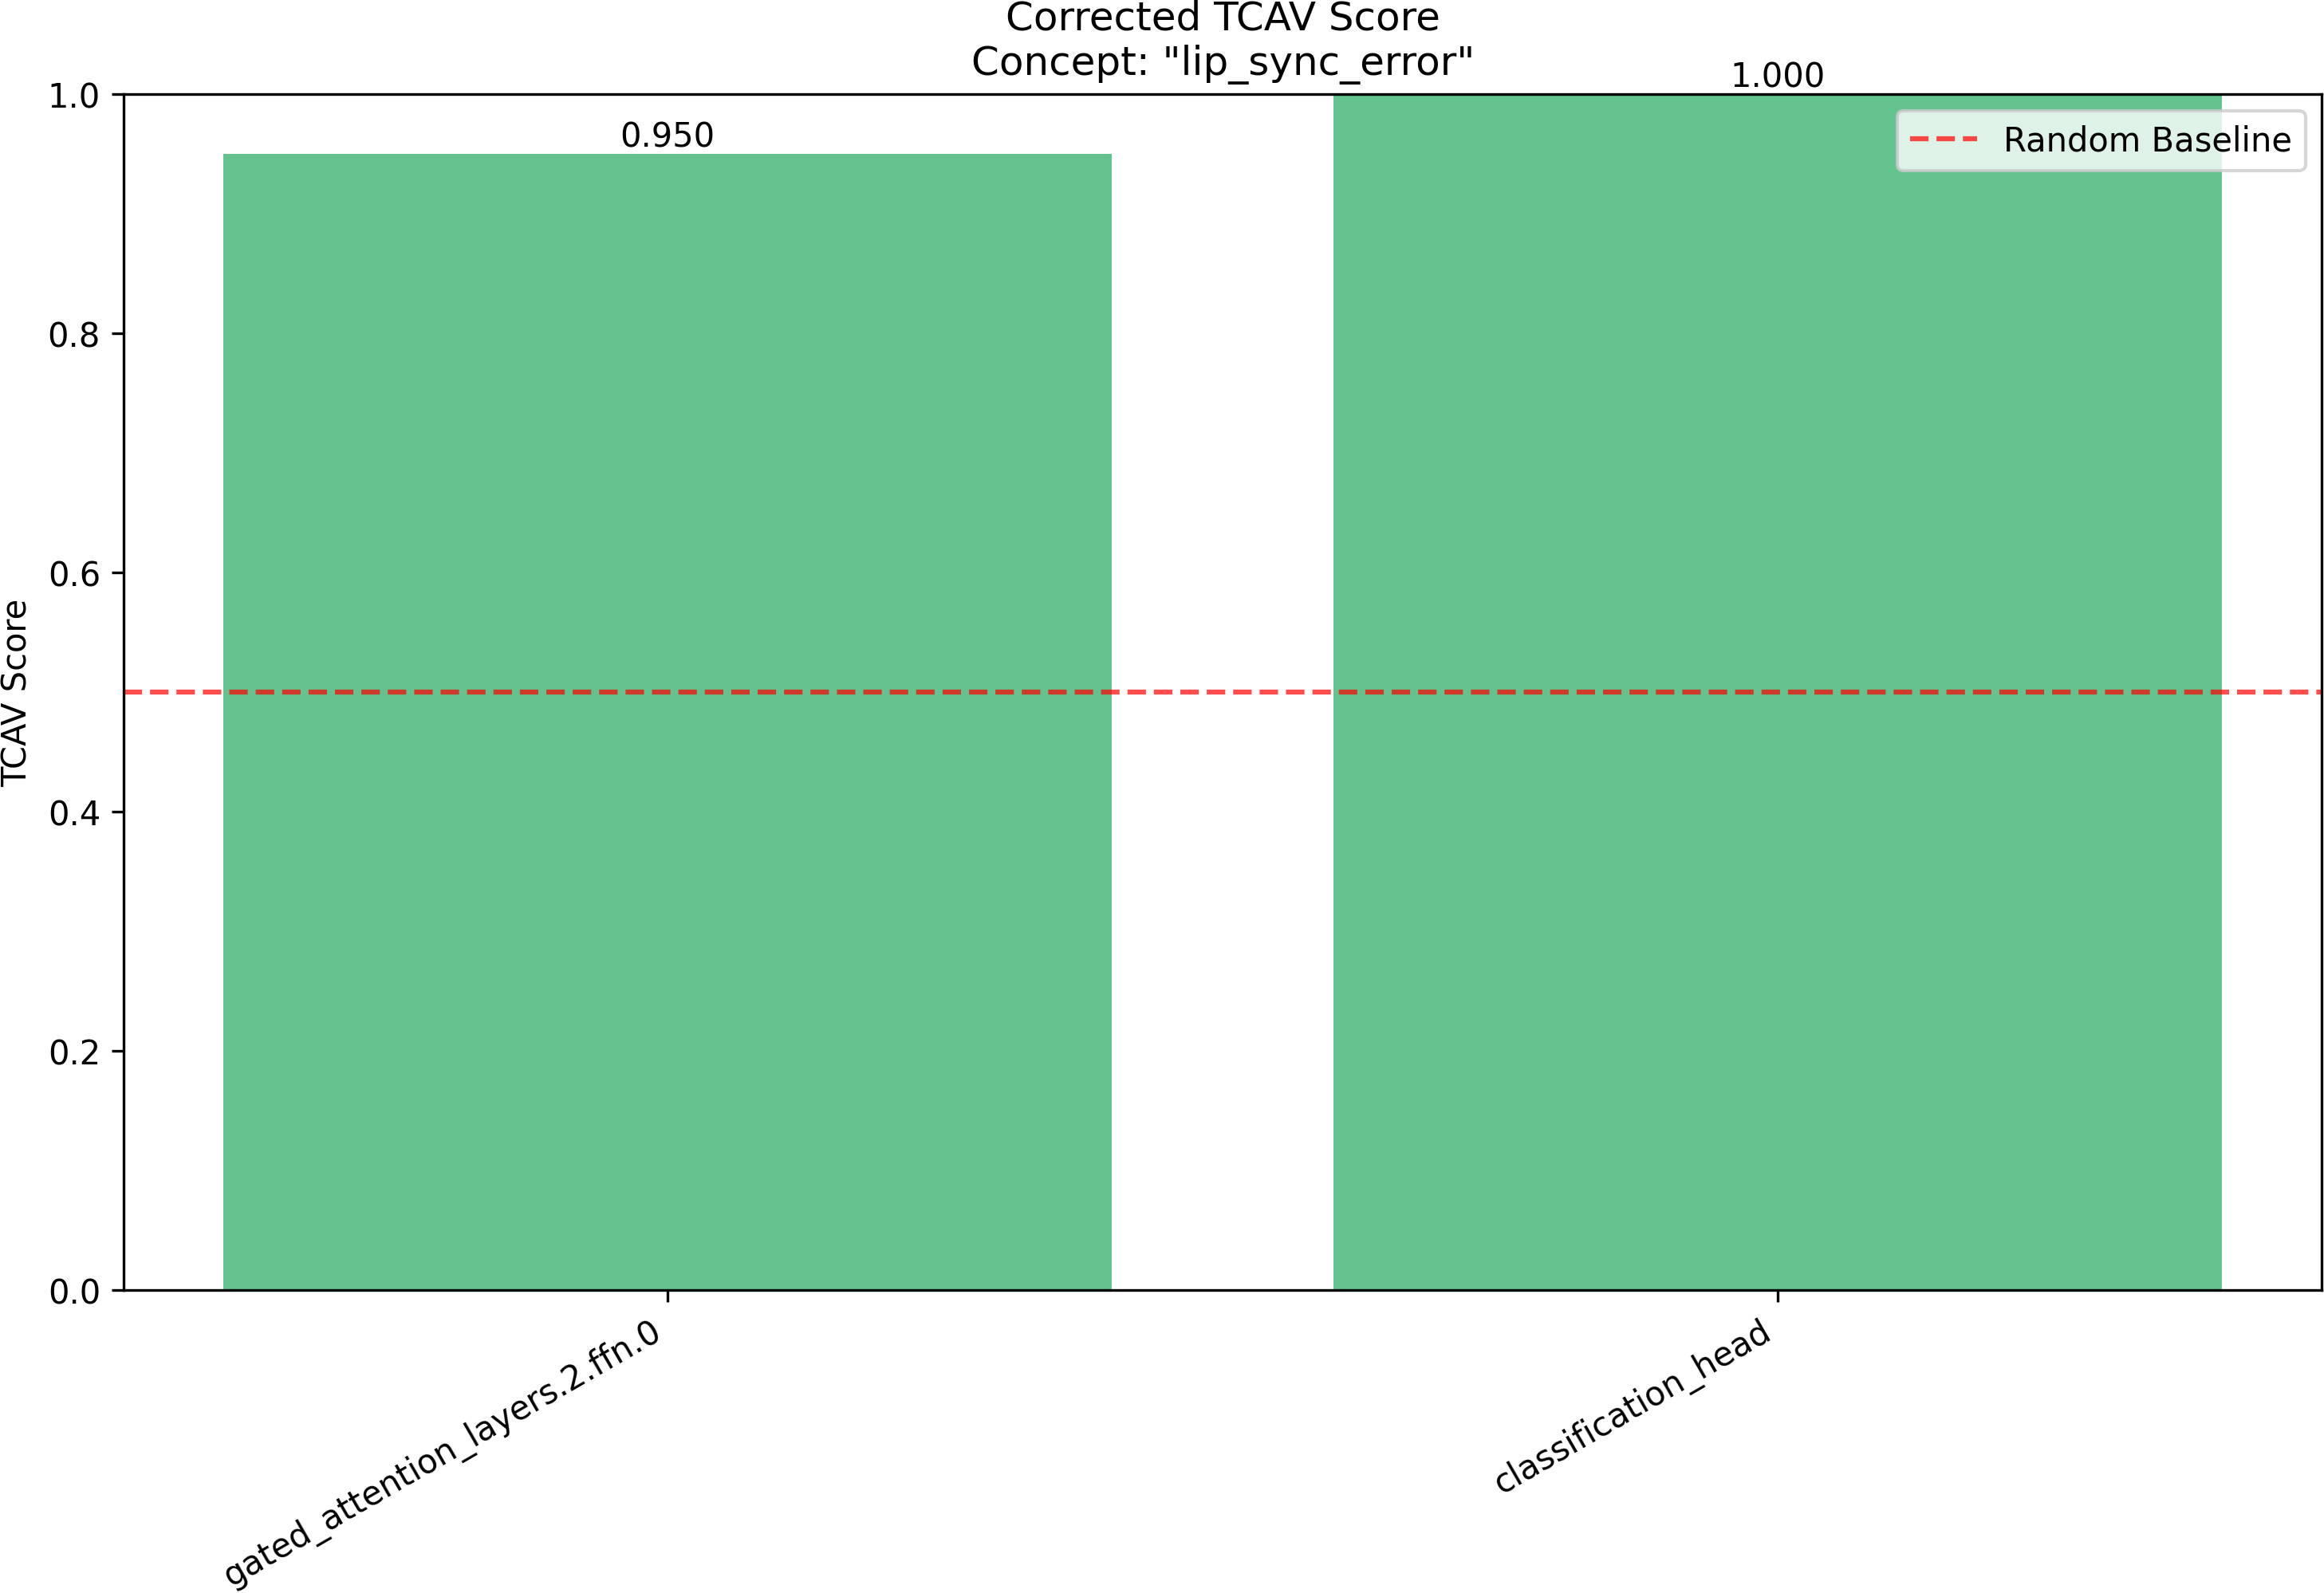
\includegraphics[width=0.72\textwidth]{image18.png}
\caption{TCAV scores for the lip-sync error concept. Scores above the random baseline indicate that the concept influences internal representations and the fake-class decision.}
\label{fig:tcav}
\end{figure}

\section{Discussion}
\label{sec:discussion}

The results support the central design claim of PinPoint: synchrony-aware supervision improves both classification performance and explanation quality. The ablation study shows that the gate, synchronization loss, and curriculum are all necessary. The no-gate model performs especially poorly on fake recall, which indicates that standard cross-attention is not enough for this task. The no-synchronization-loss model performs better than no-gate but still loses more than 22 percentage points of accuracy, showing that explicitly shaping attention structure contributes substantially to the final detector.

The XAI results also show why synchronization should be treated as part of the model design rather than as a post-hoc interpretation. In the full model, the attention map has a defined forensic meaning because it is trained to match expected audio--visual timing in aligned real samples. Attribution, counterfactual, and TCAV analyses then serve as checks on whether this learned structure agrees with visual, acoustic, and concept-level evidence. This layered explanation strategy is more informative than presenting a single heatmap after training.

PinPoint is most useful in settings where a detector must support review rather than simply return a label. A forensic analyst can inspect the predicted class, the attention structure, the visual and audio attributions, and the counterfactual sensitivity. These outputs do not eliminate the need for human judgment, but they make the model's decision pathway more transparent.

Several limitations remain. First, the current evaluation uses a unified benchmark built from curated datasets. A stronger generalization protocol should train on one dataset and test on another, and should include in-the-wild compression and social-media transformations. Second, the model uses fixed 30-frame segments, which may miss longer-range inconsistencies. Third, the full XAI suite is computationally expensive because SHAP, counterfactual generation, and gradient-based attribution require additional forward or backward passes. Fourth, the available logs do not include repeated runs or confidence intervals, so this paper avoids claims of statistical significance. Future work should add multi-seed evaluation, calibration analysis, and cross-dataset testing.

\section{Conclusions}
\label{sec:conclusion}

This paper presented PinPoint, a synchronization-aware and explainable audio--visual deepfake detector. The model combines an XAI-compatible ResNet-18 visual encoder, a CNN--GRU audio encoder, gated cross-attention, curriculum training, and a synchronization loss that shapes attention maps toward diagonal, smooth, and concentrated structures for aligned real samples.

On the unified LAV-DF and FakeAVCeleb benchmark, PinPoint achieved 97.47\% accuracy and 0.9680 macro F1 over 26,097 test samples. Ablation experiments showed that removing the gate, synchronization loss, or curriculum sharply degrades performance, confirming that synchronization-aware fusion is central to the detector. The XAI analysis showed that the full model produces more consistent explanations and that lip-sync error concepts influence internal representations and the final prediction.

The broader conclusion is that interpretability in deepfake detection should not be treated only as a post-hoc add-on. By making audio--visual synchrony part of the training objective and then auditing the resulting model with attribution, attention, counterfactual, and concept-based tools, PinPoint provides a more transparent path toward forensic multimedia analysis.

\section*{Declarations}

\textbf{Funding.} This research did not receive any specific grant from funding agencies in the public, commercial, or not-for-profit sectors.

\textbf{Competing interests.} The authors declare that they have no known competing financial interests or personal relationships that could have appeared to influence the work reported in this paper.

\textbf{Data availability.} LAV-DF and FakeAVCeleb are publicly described datasets. Derived preprocessed tensors and trained model artifacts can be made available by the authors upon reasonable request, subject to the licenses and access terms of the original datasets.

\textbf{Code availability.} The implementation is available in the project repository during review and can be released with the final manuscript subject to institutional approval.

\textbf{CRediT author statement.} Author contribution details are provided in the separate title page file to preserve double-anonymized review.

\textbf{Declaration of generative AI and AI-assisted technologies.} A disclosure statement is provided in the separate title page file for the authors to review and adjust before submission.

\begin{thebibliography}{99}

\bibitem{nguyen2024survey}
Nguyen-Le, H.H., Tran, V.T., Nguyen, D.T., Le-Khac, N.A. Passive deepfake detection across multi-modalities: A comprehensive survey. arXiv preprint arXiv:2411.17911, 2024.

\bibitem{khalid2021fakeavceleb}
Khalid, H., Tariq, S., Kim, M., Woo, S.S. FakeAVCeleb: A novel audio-video multimodal deepfake dataset. arXiv preprint arXiv:2108.05080, 2021.

\bibitem{cai2022lavdf}
Cai, Z., Stefanov, K., Dhall, A., Hayat, M. Do you really mean that? Content driven audio-visual deepfake dataset and multimodal method for temporal forgery localization. In: 2022 International Conference on Digital Image Computing: Techniques and Applications (DICTA), pp. 1--10, 2022. doi:10.1109/DICTA56598.2022.10034605.

\bibitem{chugh2020notmade}
Chugh, K., Gupta, P., Dhall, A., Subramanian, R. Not made for each other: Audio-visual dissonance-based deepfake detection and localization. In: Proceedings of the 28th ACM International Conference on Multimedia, pp. 439--447, 2020. doi:10.1145/3394171.3413700.

\bibitem{haliassos2021lips}
Haliassos, A., Vougioukas, K., Petridis, S., Pantic, M. Lips don't lie: A generalisable and robust approach to face forgery detection. In: Proceedings of the IEEE/CVF Conference on Computer Vision and Pattern Recognition, pp. 5039--5049, 2021. doi:10.1109/CVPR46437.2021.00500.

\bibitem{raza2023multimodaltrace}
Raza, M.A., Malik, K.M. Multimodaltrace: Deepfake detection using audiovisual representation learning. In: Proceedings of the IEEE/CVF Conference on Computer Vision and Pattern Recognition Workshops, pp. 993--1000, 2023. doi:10.1109/CVPRW59228.2023.00048.

\bibitem{gao2024temporal}
Gao, Y., Wang, X., Zhang, Y., Zeng, P., Ma, Y. Temporal feature prediction in audio-visual deepfake detection. Electronics 13(17), 3433, 2024. doi:10.3390/electronics13173433.

\bibitem{javed2025avsff}
Javed, M., Zhang, Z., Dahri, F.H., Laghari, A.A., Krajcik, M., Almadhor, A. Audio-visual synchronization and lip movement analysis for real-time deepfake detection. International Journal of Computational Intelligence Systems 18, 170, 2025. doi:10.1007/s44196-025-00911-7.

\bibitem{du2025cad}
Du, Y., Wang, Z., Luo, Y., Piao, C., Yan, Z., Li, H., Yuan, L. CAD: A general multimodal framework for video deepfake detection via cross-modal alignment and distillation. arXiv preprint arXiv:2505.15233, 2025.

\bibitem{koutlis2024dimodif}
Koutlis, C., Papadopoulos, S. DiMoDif: Discourse modality-information differentiation for audio-visual deepfake detection and localization. arXiv preprint arXiv:2411.10193, 2024.

\bibitem{croitoru2025mavos}
Croitoru, F.A., Hondru, V., Popescu, M., Ionescu, R.T., Khan, F.S., Shah, M. MAVOS-DD: Multilingual audio-video open-set deepfake detection benchmark. arXiv preprint arXiv:2505.11109, 2025.

\bibitem{kaya2026integrated}
Kaya, M., Alhajj, R. An integrated explainable framework for multimodal deepfake detection across image, audio, and video data. Ain Shams Engineering Journal 17(7), 104233, 2026. doi:10.1016/j.asej.2026.104233.

\bibitem{ribeiro2016lime}
Ribeiro, M.T., Singh, S., Guestrin, C. Why should I trust you? Explaining the predictions of any classifier. In: Proceedings of the 22nd ACM SIGKDD International Conference on Knowledge Discovery and Data Mining, pp. 1135--1144, 2016. doi:10.1145/2939672.2939778.

\bibitem{lundberg2017shap}
Lundberg, S.M., Lee, S.I. A unified approach to interpreting model predictions. In: Advances in Neural Information Processing Systems 30, pp. 4765--4774, 2017.

\bibitem{sundararajan2017ig}
Sundararajan, M., Taly, A., Yan, Q. Axiomatic attribution for deep networks. In: Proceedings of the 34th International Conference on Machine Learning, pp. 3319--3328, 2017.

\bibitem{bach2015lrp}
Bach, S., Binder, A., Montavon, G., Klauschen, F., Muller, K.R., Samek, W. On pixel-wise explanations for non-linear classifier decisions by layer-wise relevance propagation. PLOS ONE 10(7), e0130140, 2015. doi:10.1371/journal.pone.0130140.

\bibitem{selvaraju2017gradcam}
Selvaraju, R.R., Cogswell, M., Das, A., Vedantam, R., Parikh, D., Batra, D. Grad-CAM: Visual explanations from deep networks via gradient-based localization. In: Proceedings of the IEEE International Conference on Computer Vision, pp. 618--626, 2017. doi:10.1109/ICCV.2017.74.

\bibitem{kim2018tcav}
Kim, B., Wattenberg, M., Gilmer, J., Cai, C., Wexler, J., Viegas, F., Sayres, R. Interpretability beyond feature attribution: Quantitative testing with concept activation vectors (TCAV). In: Proceedings of the 35th International Conference on Machine Learning, pp. 2668--2677, 2018.

\bibitem{baldassarre2022metrics}
Baldassarre, F., Debard, Q., Pontiveros, G.F., Wijaya, T.K. Quantitative metrics for evaluating explanations of video DeepFake detectors. In: Proceedings of the British Machine Vision Conference, 2022. arXiv:2210.03683.

\bibitem{tsigos2024xai}
Tsigos, K., Apostolidis, E., Baxevanakis, S., Papadopoulos, S., Mezaris, V. Towards quantitative evaluation of explainable AI methods for deepfake detection. In: Proceedings of the 3rd ACM International Workshop on Multimedia AI against Disinformation, pp. 37--45, 2024. doi:10.1145/3643491.3660292.

\bibitem{he2016resnet}
He, K., Zhang, X., Ren, S., Sun, J. Deep residual learning for image recognition. In: Proceedings of the IEEE Conference on Computer Vision and Pattern Recognition, pp. 770--778, 2016. doi:10.1109/CVPR.2016.90.

\end{thebibliography}

\end{document}
